\documentclass[10pt]{article}
\usepackage{tikz}
\usepackage[margin=0cm]{geometry}
\pagestyle{empty}

\begin{document}

\vspace*{\fill}
\begin{center}
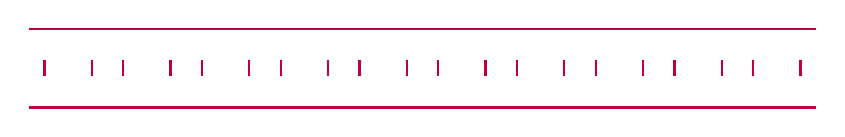
\begin{tikzpicture}[x=0.2cm, y=-0.2cm, thick, purple]
% North to South lines
    \draw (1,2) -- (1,3);
    \draw (4,2) -- (4,3);
    \draw (6,2) -- (6,3);
    \draw (9,2) -- (9,3);
    \draw (11,2) -- (11,3);
    \draw (14,2) -- (14,3);
    \draw (16,2) -- (16,3);
    \draw (19,2) -- (19,3);
    \draw (21,2) -- (21,3);
    \draw (24,2) -- (24,3);
    \draw (26,2) -- (26,3);
    \draw (29,2) -- (29,3);
    \draw (31,2) -- (31,3);
    \draw (34,2) -- (34,3);
    \draw (36,2) -- (36,3);
    \draw (39,2) -- (39,3);
    \draw (41,2) -- (41,3);
    \draw (44,2) -- (44,3);
    \draw (46,2) -- (46,3);
    \draw (49,2) -- (49,3);
% North-West to South-East lines
% West to East lines
    \draw (0,0) -- (50,0);
    \draw (0,5) -- (50,5);
% South-West to North-East lines
\end{tikzpicture}
\end{center}
\vspace*{\fill}

\end{document}
